\vspace{-0.5cm}
The Immelmann turn, named after German World War I flying ace Max Immelmann, is an an  aerobatic maneuver that results in level-flight of the aircraft in the opposite direction and higher altitude.

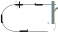
\includegraphics[width=\linewidth]{figures/immelmann-overview}
\captionof{figure}{Immelmann turn overview. Own elaboration.}
\label{fig:immelmann-overview}
\vspace*{0.5cm}

The aircraft initiates this maneuver in straight levelled flight, and describes an upwards semicircle contained in its symmetry plane. This increases the flight altitude while changing the trajectory's to the original's opposite direction and leaves the plane turned upside down. It then rolls while still flying in a straigth line, and returns to the initial condition of levelled flight.\\

This maneuver can be performed for various velocities and radius, but there are some dependencies and limitiations to be taken into account, such as the maximum deflections or forces the control surfaces can provide or support, respectively.

In order to cover all these variables, a first approach through the dynamic and kinetic equations follows.

